\documentclass{standalone}

\usepackage[english]{babel} % English language/hyphenation
\usepackage{clock} % Required for generation clock icon
\ClockFrametrue\ClockStyle=3 % Format the clock icons
\usepackage{gensymb} % gives the degree symbol
\usepackage{graphicx} % Required for including pictures
\usepackage{tikz} % Required for drawing custom shapes
\usetikzlibrary{arrows}
\usetikzlibrary{shapes.misc}
\usetikzlibrary{decorations.pathreplacing}

\definecolor{gridgray}{RGB}{192,192,192}
\definecolor{medgray}{RGB}{128,128,128}
\definecolor{redback}{RGB}{255,168,168}
\definecolor{redback2}{RGB}{128,0,0}
\definecolor{greenback}{RGB}{168,255,168}
\definecolor{greenpastel}{RGB}{210,255,210}
\definecolor{greenback2}{RGB}{0,192,0}
\definecolor{darkgreenback}{RGB}{0,96,0}
\definecolor{yellowback}{RGB}{255,255,168}
\definecolor{darkyellowback}{RGB}{96,96,0}
\definecolor{orangeback}{RGB}{255,192,128}
\definecolor{orangeback2}{RGB}{255,220,192}
\definecolor{darkorangeback}{RGB}{128,54,0}
\definecolor{yellowback2}{RGB}{255,255,192}
\definecolor{aquaback}{RGB}{192,255,255}
\definecolor{darkaquaback}{RGB}{0,96,96}
\definecolor{blueback}{RGB}{168,168,255}
\definecolor{magentaback}{RGB}{255,210,255}
\definecolor{darkmagentaback}{RGB}{96,0,96}

\begin{document}
	\def\glider#1#2#3{
		\begin{scope}[shift={#1}, rotate=#2, scale=#3]
			\fill[black](0,0) -- (1,0) -- (1,1) -- (0,1) -- cycle;
			\fill[black](8/7+0,0) -- (8/7+1,0) -- (8/7+1,1) -- (8/7+0,1) -- cycle;
			\fill[black](16/7+0,0) -- (16/7+1,0) -- (16/7+1,1) -- (16/7+0,1) -- cycle;
			\fill[black](16/7+0,8/7+0) -- (16/7+1,8/7+0) -- (16/7+1,8/7+1) -- (16/7+0,8/7+1) -- cycle;
			\fill[black](8/7+0,16/7+0) -- (8/7+1,16/7+0) -- (8/7+1,16/7+1) -- (8/7+0,16/7+1) -- cycle;
		\end{scope}
	}
	\def\lwss#1#2#3{
		\begin{scope}[shift={#1}, rotate=#2, scale=#3]
			\fill[black](0,0) -- (1,0) -- (1,1) -- (0,1) -- cycle;
			\fill[black](8/7+0,0) -- (8/7+1,0) -- (8/7+1,1) -- (8/7+0,1) -- cycle;
			\fill[black](16/7+0,0) -- (16/7+1,0) -- (16/7+1,1) -- (16/7+0,1) -- cycle;
			\fill[black](24/7+0,0) -- (24/7+1,0) -- (24/7+1,1) -- (24/7+0,1) -- cycle;
			\fill[black](32/7+0,8/7+0) -- (32/7+1,8/7+0) -- (32/7+1,8/7+1) -- (32/7+0,8/7+1) -- cycle;
			\fill[black](0,8/7+0) -- (1,8/7+0) -- (1,8/7+1) -- (0,8/7+1) -- cycle;
			\fill[black](0,16/7+0) -- (1,16/7+0) -- (1,16/7+1) -- (0,16/7+1) -- cycle;
			\fill[black](8/7+0,24/7+0) -- (8/7+1,24/7+0) -- (8/7+1,24/7+1) -- (8/7+0,24/7+1) -- cycle;
			\fill[black](32/7+0,24/7+0) -- (32/7+1,24/7+0) -- (32/7+1,24/7+1) -- (32/7+0,24/7+1) -- cycle;
		\end{scope}
	}
	\def\mwss#1#2#3{
		\begin{scope}[shift={#1}, rotate=#2, scale=#3]
			\fill[black](0,0) -- (1,0) -- (1,1) -- (0,1) -- cycle;
			\fill[black](8/7+0,0) -- (8/7+1,0) -- (8/7+1,1) -- (8/7+0,1) -- cycle;
			\fill[black](16/7+0,0) -- (16/7+1,0) -- (16/7+1,1) -- (16/7+0,1) -- cycle;
			\fill[black](24/7+0,0) -- (24/7+1,0) -- (24/7+1,1) -- (24/7+0,1) -- cycle;
			\fill[black](32/7+0,0) -- (32/7+1,0) -- (32/7+1,1) -- (32/7+0,1) -- cycle;
			\fill[black](40/7+0,8/7+0) -- (40/7+1,8/7+0) -- (40/7+1,8/7+1) -- (40/7+0,8/7+1) -- cycle;
			\fill[black](0,8/7+0) -- (1,8/7+0) -- (1,8/7+1) -- (0,8/7+1) -- cycle;
			\fill[black](0,16/7+0) -- (1,16/7+0) -- (1,16/7+1) -- (0,16/7+1) -- cycle;
			\fill[black](8/7+0,24/7+0) -- (8/7+1,24/7+0) -- (8/7+1,24/7+1) -- (8/7+0,24/7+1) -- cycle;
			\fill[black](24/7+0,32/7+0) -- (24/7+1,32/7+0) -- (24/7+1,32/7+1) -- (24/7+0,32/7+1) -- cycle;
			\fill[black](40/7+0,24/7+0) -- (40/7+1,24/7+0) -- (40/7+1,24/7+1) -- (40/7+0,24/7+1) -- cycle;
		\end{scope}
	}
	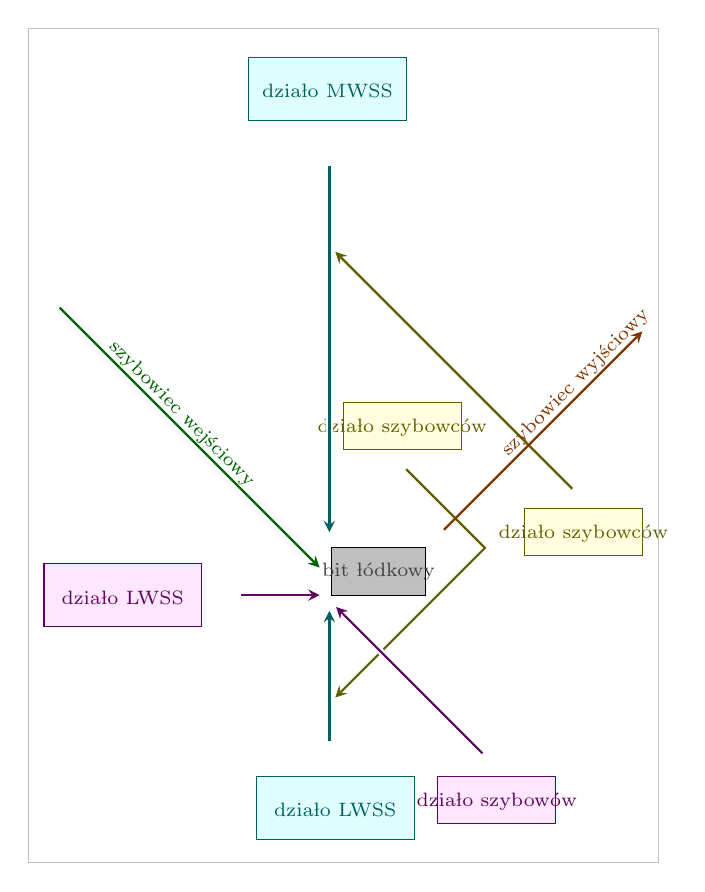
\begin{tikzpicture}%
		% LWSS GUN LEFT
		\filldraw[color=darkmagentaback,fill=magentaback!50] (0,-1.2) -- (2,-1.2) -- (2,-2) -- (0,-2) -- cycle;
		\draw[darkmagentaback] (1,-2.13+0.5) node {\scriptsize działo LWSS};
		\draw[thick,color=darkmagentaback,-stealth] (2.5,-1.6) -- (3.5,-1.6);
		\lwss{(2.5,-1.465)}{180}{0.08};
		
		% GLIDER GUN TOP RIGHT
		\filldraw[color=darkyellowback,fill=yellowback2!50] (3.8,0.85) rectangle (5.3,0.25);
		\draw[darkyellowback] (4.55,0.53) node {\scriptsize działo szybowców};
		\draw[thick,color=darkyellowback,-stealth] (4.6,0) -- (5.6,-1) -- (3.7,-2.9);
		\glider{(4.4,-0.06)}{0}{0.08};
		
		% MWSS GUN TOP
		\filldraw[color=darkaquaback,fill=aquaback!50] (2.6,4.43) -- (4.6,4.43) -- (4.6,5.23) -- (2.6,5.23) -- cycle;
		\draw[darkaquaback] (3.6,4.8) node {\scriptsize działo MWSS};
		\draw[line width=2.4pt,color=white,-stealth] (3.625,3.85) -- (3.625,-0.8); % since this stream passes over another one
		\draw[thick,color=darkaquaback,-stealth] (3.625,3.85) -- (3.625,-0.8);
		\mwss{(3.756,3.85)}{90}{0.08};

		% BOAT-BIT
		\filldraw[color=black,fill=gray!50] (3.65,-1) -- (4.85,-1) -- (4.85,-1.6) -- (3.65,-1.6) -- cycle;
		\draw[darkgray] (4.25,-1.3) node {\scriptsize bit łódkowy};

		% LWSS GUN BOTTOM
		\filldraw[color=darkaquaback,fill=aquaback!50] (2.7,-3.9) -- (4.7,-3.9) -- (4.7,-4.7) -- (2.7,-4.7) -- cycle;
		\draw[darkaquaback] (3.7,-4.83+0.5) node {\scriptsize działo LWSS};
		\draw[thick,color=darkaquaback,-stealth] (3.625,-3.45) -- (3.625,-1.8);
		\lwss{(3.5,-3.4)}{270}{0.08};
		
		% GLIDER GUN BOTTOM
		\filldraw[color=darkmagentaback,fill=magentaback!50] (5,-3.9) -- (6.5,-3.9) -- (6.5,-4.5) -- (5,-4.5) -- cycle;
		\draw[darkmagentaback] (5.75,-4.22) node {\scriptsize działo szybowów};
		\draw[line width=2.4pt,color=white,-stealth] (5.61,-3.65) -- (3.71,-1.75); % since this stream passes over another one
		\draw[thick,color=darkmagentaback,-stealth] (5.57,-3.61) -- (3.71,-1.75);
		\glider{(5.8,-3.58)}{180}{0.08};
		
		% GLIDER GUN BOTTOM RIGHT
		\filldraw[color=darkyellowback,fill=yellowback2!50] (6.1,-0.5) -- (7.6,-0.5) -- (7.6,-1.1) -- (6.1,-1.1) -- cycle;
		\draw[darkyellowback] (6.85,-0.82) node {\scriptsize działo szybowców};
		\draw[thick,color=darkyellowback,-stealth] (6.71,-0.25) -- (3.7,2.76);
		\glider{(6.9,-0.18)}{180}{0.08};
		
		% OUTPUT GLIDER
		\draw[thick,color=darkorangeback,-stealth] (5.08,-0.77) -- (7.6,1.75);
		\draw[darkorangeback] (6.75,1.1) node[rotate=45] {\scriptsize szybowiec wyjściowy};
		\glider{(5.1,-1)}{90}{0.08};
		
		% INPUT GLIDER
		\draw[thick,color=darkgreenback,-stealth] (0.2,2.05) -- (3.5,-1.25);
		\draw[darkgreenback] (1.75,0.7) node[rotate=-45] {\scriptsize szybowiec wejściowy};
		\glider{(-0.049,2.04)}{0}{0.08};
		
		% BORDER
		\draw[gridgray] (-0.2,5.6) -- (7.8,5.6) -- (7.8,-5) -- (-0.2,-5) -- cycle;
	\end{tikzpicture}
\end{document}
